% Options for packages loaded elsewhere
% Options for packages loaded elsewhere
\PassOptionsToPackage{unicode}{hyperref}
\PassOptionsToPackage{hyphens}{url}
\PassOptionsToPackage{dvipsnames,svgnames,x11names}{xcolor}
%
\documentclass[
  letterpaper,
  DIV=11,
  numbers=noendperiod]{scrartcl}
\usepackage{xcolor}
\usepackage{amsmath,amssymb}
\setcounter{secnumdepth}{-\maxdimen} % remove section numbering
\usepackage{iftex}
\ifPDFTeX
  \usepackage[T1]{fontenc}
  \usepackage[utf8]{inputenc}
  \usepackage{textcomp} % provide euro and other symbols
\else % if luatex or xetex
  \usepackage{unicode-math} % this also loads fontspec
  \defaultfontfeatures{Scale=MatchLowercase}
  \defaultfontfeatures[\rmfamily]{Ligatures=TeX,Scale=1}
\fi
\usepackage{lmodern}
\ifPDFTeX\else
  % xetex/luatex font selection
  \setmainfont[]{Times New Roman}
\fi
% Use upquote if available, for straight quotes in verbatim environments
\IfFileExists{upquote.sty}{\usepackage{upquote}}{}
\IfFileExists{microtype.sty}{% use microtype if available
  \usepackage[]{microtype}
  \UseMicrotypeSet[protrusion]{basicmath} % disable protrusion for tt fonts
}{}
\makeatletter
\@ifundefined{KOMAClassName}{% if non-KOMA class
  \IfFileExists{parskip.sty}{%
    \usepackage{parskip}
  }{% else
    \setlength{\parindent}{0pt}
    \setlength{\parskip}{6pt plus 2pt minus 1pt}}
}{% if KOMA class
  \KOMAoptions{parskip=half}}
\makeatother
% Make \paragraph and \subparagraph free-standing
\makeatletter
\ifx\paragraph\undefined\else
  \let\oldparagraph\paragraph
  \renewcommand{\paragraph}{
    \@ifstar
      \xxxParagraphStar
      \xxxParagraphNoStar
  }
  \newcommand{\xxxParagraphStar}[1]{\oldparagraph*{#1}\mbox{}}
  \newcommand{\xxxParagraphNoStar}[1]{\oldparagraph{#1}\mbox{}}
\fi
\ifx\subparagraph\undefined\else
  \let\oldsubparagraph\subparagraph
  \renewcommand{\subparagraph}{
    \@ifstar
      \xxxSubParagraphStar
      \xxxSubParagraphNoStar
  }
  \newcommand{\xxxSubParagraphStar}[1]{\oldsubparagraph*{#1}\mbox{}}
  \newcommand{\xxxSubParagraphNoStar}[1]{\oldsubparagraph{#1}\mbox{}}
\fi
\makeatother

\usepackage{color}
\usepackage{fancyvrb}
\newcommand{\VerbBar}{|}
\newcommand{\VERB}{\Verb[commandchars=\\\{\}]}
\DefineVerbatimEnvironment{Highlighting}{Verbatim}{commandchars=\\\{\}}
% Add ',fontsize=\small' for more characters per line
\usepackage{framed}
\definecolor{shadecolor}{RGB}{241,243,245}
\newenvironment{Shaded}{\begin{snugshade}}{\end{snugshade}}
\newcommand{\AlertTok}[1]{\textcolor[rgb]{0.68,0.00,0.00}{#1}}
\newcommand{\AnnotationTok}[1]{\textcolor[rgb]{0.37,0.37,0.37}{#1}}
\newcommand{\AttributeTok}[1]{\textcolor[rgb]{0.40,0.45,0.13}{#1}}
\newcommand{\BaseNTok}[1]{\textcolor[rgb]{0.68,0.00,0.00}{#1}}
\newcommand{\BuiltInTok}[1]{\textcolor[rgb]{0.00,0.23,0.31}{#1}}
\newcommand{\CharTok}[1]{\textcolor[rgb]{0.13,0.47,0.30}{#1}}
\newcommand{\CommentTok}[1]{\textcolor[rgb]{0.37,0.37,0.37}{#1}}
\newcommand{\CommentVarTok}[1]{\textcolor[rgb]{0.37,0.37,0.37}{\textit{#1}}}
\newcommand{\ConstantTok}[1]{\textcolor[rgb]{0.56,0.35,0.01}{#1}}
\newcommand{\ControlFlowTok}[1]{\textcolor[rgb]{0.00,0.23,0.31}{\textbf{#1}}}
\newcommand{\DataTypeTok}[1]{\textcolor[rgb]{0.68,0.00,0.00}{#1}}
\newcommand{\DecValTok}[1]{\textcolor[rgb]{0.68,0.00,0.00}{#1}}
\newcommand{\DocumentationTok}[1]{\textcolor[rgb]{0.37,0.37,0.37}{\textit{#1}}}
\newcommand{\ErrorTok}[1]{\textcolor[rgb]{0.68,0.00,0.00}{#1}}
\newcommand{\ExtensionTok}[1]{\textcolor[rgb]{0.00,0.23,0.31}{#1}}
\newcommand{\FloatTok}[1]{\textcolor[rgb]{0.68,0.00,0.00}{#1}}
\newcommand{\FunctionTok}[1]{\textcolor[rgb]{0.28,0.35,0.67}{#1}}
\newcommand{\ImportTok}[1]{\textcolor[rgb]{0.00,0.46,0.62}{#1}}
\newcommand{\InformationTok}[1]{\textcolor[rgb]{0.37,0.37,0.37}{#1}}
\newcommand{\KeywordTok}[1]{\textcolor[rgb]{0.00,0.23,0.31}{\textbf{#1}}}
\newcommand{\NormalTok}[1]{\textcolor[rgb]{0.00,0.23,0.31}{#1}}
\newcommand{\OperatorTok}[1]{\textcolor[rgb]{0.37,0.37,0.37}{#1}}
\newcommand{\OtherTok}[1]{\textcolor[rgb]{0.00,0.23,0.31}{#1}}
\newcommand{\PreprocessorTok}[1]{\textcolor[rgb]{0.68,0.00,0.00}{#1}}
\newcommand{\RegionMarkerTok}[1]{\textcolor[rgb]{0.00,0.23,0.31}{#1}}
\newcommand{\SpecialCharTok}[1]{\textcolor[rgb]{0.37,0.37,0.37}{#1}}
\newcommand{\SpecialStringTok}[1]{\textcolor[rgb]{0.13,0.47,0.30}{#1}}
\newcommand{\StringTok}[1]{\textcolor[rgb]{0.13,0.47,0.30}{#1}}
\newcommand{\VariableTok}[1]{\textcolor[rgb]{0.07,0.07,0.07}{#1}}
\newcommand{\VerbatimStringTok}[1]{\textcolor[rgb]{0.13,0.47,0.30}{#1}}
\newcommand{\WarningTok}[1]{\textcolor[rgb]{0.37,0.37,0.37}{\textit{#1}}}

\usepackage{longtable,booktabs,array}
\newcounter{none} % for unnumbered tables
\usepackage{calc} % for calculating minipage widths
% Correct order of tables after \paragraph or \subparagraph
\usepackage{etoolbox}
\makeatletter
\patchcmd\longtable{\par}{\if@noskipsec\mbox{}\fi\par}{}{}
\makeatother
% Allow footnotes in longtable head/foot
\IfFileExists{footnotehyper.sty}{\usepackage{footnotehyper}}{\usepackage{footnote}}
\makesavenoteenv{longtable}
\usepackage{graphicx}
\makeatletter
\newsavebox\pandoc@box
\newcommand*\pandocbounded[1]{% scales image to fit in text height/width
  \sbox\pandoc@box{#1}%
  \Gscale@div\@tempa{\textheight}{\dimexpr\ht\pandoc@box+\dp\pandoc@box\relax}%
  \Gscale@div\@tempb{\linewidth}{\wd\pandoc@box}%
  \ifdim\@tempb\p@<\@tempa\p@\let\@tempa\@tempb\fi% select the smaller of both
  \ifdim\@tempa\p@<\p@\scalebox{\@tempa}{\usebox\pandoc@box}%
  \else\usebox{\pandoc@box}%
  \fi%
}
% Set default figure placement to htbp
\def\fps@figure{htbp}
\makeatother





\setlength{\emergencystretch}{3em} % prevent overfull lines

\providecommand{\tightlist}{%
  \setlength{\itemsep}{0pt}\setlength{\parskip}{0pt}}



 


\KOMAoption{captions}{tableheading}
\makeatletter
\@ifpackageloaded{caption}{}{\usepackage{caption}}
\AtBeginDocument{%
\ifdefined\contentsname
  \renewcommand*\contentsname{Table of contents}
\else
  \newcommand\contentsname{Table of contents}
\fi
\ifdefined\listfigurename
  \renewcommand*\listfigurename{List of Figures}
\else
  \newcommand\listfigurename{List of Figures}
\fi
\ifdefined\listtablename
  \renewcommand*\listtablename{List of Tables}
\else
  \newcommand\listtablename{List of Tables}
\fi
\ifdefined\figurename
  \renewcommand*\figurename{Figure}
\else
  \newcommand\figurename{Figure}
\fi
\ifdefined\tablename
  \renewcommand*\tablename{Table}
\else
  \newcommand\tablename{Table}
\fi
}
\@ifpackageloaded{float}{}{\usepackage{float}}
\floatstyle{ruled}
\@ifundefined{c@chapter}{\newfloat{codelisting}{h}{lop}}{\newfloat{codelisting}{h}{lop}[chapter]}
\floatname{codelisting}{Listing}
\newcommand*\listoflistings{\listof{codelisting}{List of Listings}}
\makeatother
\makeatletter
\makeatother
\makeatletter
\@ifpackageloaded{caption}{}{\usepackage{caption}}
\@ifpackageloaded{subcaption}{}{\usepackage{subcaption}}
\makeatother
\usepackage{bookmark}
\IfFileExists{xurl.sty}{\usepackage{xurl}}{} % add URL line breaks if available
\urlstyle{same}
\hypersetup{
  pdftitle={Homework 3 - 193DS Spring},
  pdfauthor={Michael Torbensen},
  colorlinks=true,
  linkcolor={blue},
  filecolor={Maroon},
  citecolor={Blue},
  urlcolor={Blue},
  pdfcreator={LaTeX via pandoc}}


\title{Homework 3 - 193DS Spring}
\author{Michael Torbensen}
\date{2026-05-26}
\begin{document}
\maketitle

\renewcommand*\contentsname{Table of contents}
{
\setcounter{tocdepth}{3}
\tableofcontents
}

\begin{Shaded}
\begin{Highlighting}[]
\CommentTok{\# attaching packages }

\FunctionTok{library}\NormalTok{(tidyverse)}
\FunctionTok{library}\NormalTok{(janitor)}
\FunctionTok{library}\NormalTok{(here)}
\FunctionTok{library}\NormalTok{(effectsize)}
\FunctionTok{library}\NormalTok{(readxl)}
\FunctionTok{library}\NormalTok{ (ggeffects)}
\FunctionTok{library}\NormalTok{(rstatix)}

\CommentTok{\# reading in kelp data }
\NormalTok{kelp }\OtherTok{\textless{}{-}} \FunctionTok{read.csv}\NormalTok{(}
  \FunctionTok{here}\NormalTok{(}\StringTok{"data"}\NormalTok{, }\StringTok{"temp\_kelp.csv"}\NormalTok{))}

\CommentTok{\# reading in personal data }
\NormalTok{my\_data }\OtherTok{\textless{}{-}} \FunctionTok{read.csv}\NormalTok{(}
  \FunctionTok{here}\NormalTok{(}\StringTok{"data"}\NormalTok{,}\StringTok{"personal\_data.csv"}\NormalTok{))}
\end{Highlighting}
\end{Shaded}

\section{Problem 1. Giant Kelp
Fronds}\label{problem-1.-giant-kelp-fronds}

\subsection{a. An appropraite test}\label{a.-an-appropraite-test}

To start off, in order to measure the strength and direction of the
relationship between kelp length and temperature I will use Pearson's
Correlation Coefficient. Another good test to add could be the simple
linear regression test as it can clarify if a true linear relationship
exists between the two variables. In order to visualize and model the
relationship, I will use a simple linear regression model. The Pearson's
Correlation Coefficient provides a numerical value to describe the
relationship between the two variables and the simple linear regression
models this relationship with a line.

\subsection{b. Create a visualization}\label{b.-create-a-visualization}

\begin{Shaded}
\begin{Highlighting}[]
\CommentTok{\# base layer: ggplot}
\FunctionTok{ggplot}\NormalTok{(}\AttributeTok{data =}\NormalTok{ kelp, }
       \CommentTok{\# x{-}axis: temperature}
       \CommentTok{\# y{-}axis: kelp elongation rate (cm/day)}
       \AttributeTok{mapping =} \FunctionTok{aes}\NormalTok{(}\AttributeTok{x =}\NormalTok{ temp\_c,}
                     \AttributeTok{y =}\NormalTok{ kelp\_elong)) }\SpecialCharTok{+}
  \CommentTok{\# first layer: adding data points }
  \FunctionTok{geom\_point}\NormalTok{(}\AttributeTok{color =} \StringTok{"\#2a9d8f"}\NormalTok{,}
             \AttributeTok{alpha =} \FloatTok{0.7}\NormalTok{,}
             \AttributeTok{size =} \DecValTok{3}\NormalTok{) }\SpecialCharTok{+}
  \CommentTok{\# labeling x{-} and y{-}axis }
  \FunctionTok{labs}\NormalTok{(}
    \AttributeTok{x =} \StringTok{"Temperature (°C)"}\NormalTok{,}
    \AttributeTok{y =} \StringTok{"Frond Elongation Rate (cm/day)"}\NormalTok{, }
    \AttributeTok{title =} \StringTok{"Average Giant Kelp Frond Growth in Different Temperatures"}\NormalTok{) }\SpecialCharTok{+}
  \CommentTok{\# adding different theme from default}
  \FunctionTok{theme\_minimal}\NormalTok{()}
\end{Highlighting}
\end{Shaded}

\pandocbounded{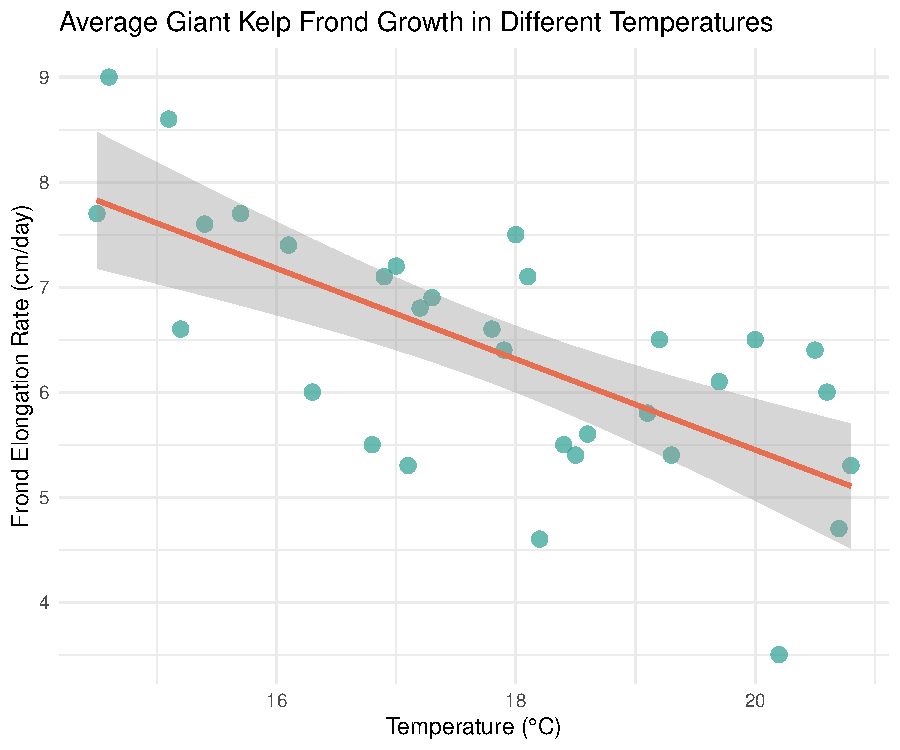
\includegraphics[keepaspectratio]{Homework_quarto_doc_files/figure-pdf/unnamed-chunk-2-1.pdf}}

\subsection{c.~Checking assumptions and running
tests}\label{c.-checking-assumptions-and-running-tests}

\subsubsection{1. Checking assumptions}\label{checking-assumptions}

\begin{Shaded}
\begin{Highlighting}[]
\CommentTok{\# Fit the model first to extract residuals}
\NormalTok{kelp\_model }\OtherTok{\textless{}{-}} \FunctionTok{lm}\NormalTok{(}
\NormalTok{  kelp\_elong }\SpecialCharTok{\textasciitilde{}}\NormalTok{ temp\_c,}
  \AttributeTok{data =}\NormalTok{ kelp) }

\CommentTok{\# Check normality of residuals: Q{-}Q plot}
\FunctionTok{qqnorm}\NormalTok{(}\FunctionTok{residuals}\NormalTok{(kelp\_model))}
\FunctionTok{qqline}\NormalTok{(}\FunctionTok{residuals}\NormalTok{(kelp\_model),}
       \AttributeTok{col =} \StringTok{"\#e76f51"}\NormalTok{)}
\end{Highlighting}
\end{Shaded}

\pandocbounded{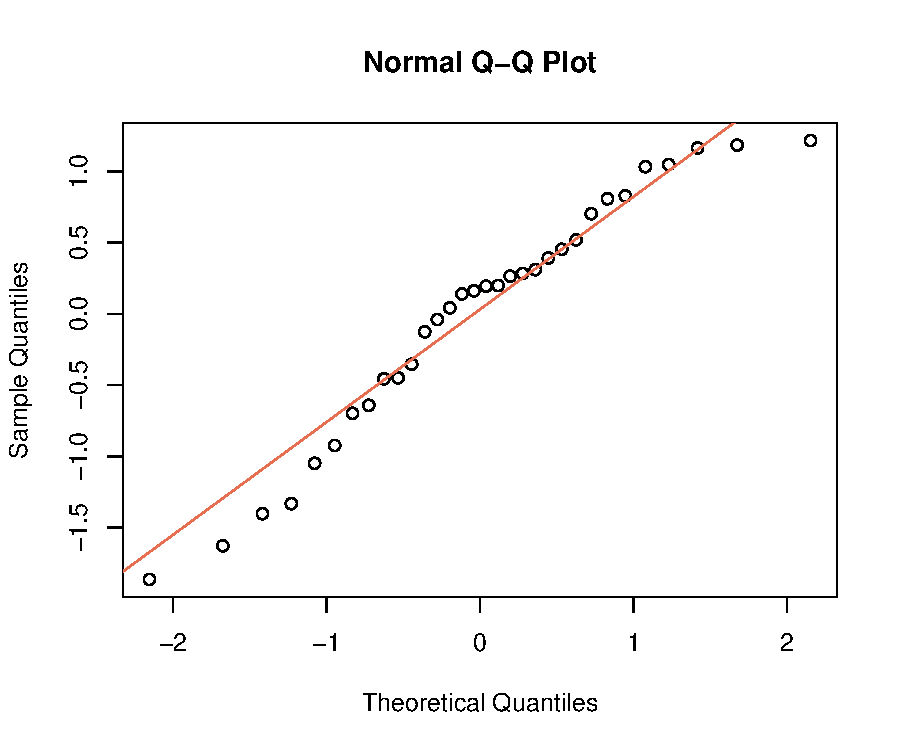
\includegraphics[keepaspectratio]{Homework_quarto_doc_files/figure-pdf/unnamed-chunk-3-1.pdf}}

\begin{Shaded}
\begin{Highlighting}[]
\CommentTok{\# Check homoscedasticity: residuals vs fitted values }
\FunctionTok{plot}\NormalTok{(}\FunctionTok{fitted}\NormalTok{(kelp\_model),}
     \FunctionTok{residuals}\NormalTok{(kelp\_model),}
     \AttributeTok{xlab =} \StringTok{"Fitted values"}\NormalTok{, }
     \AttributeTok{ylab =} \StringTok{"Residuals"}\NormalTok{, }
     \AttributeTok{pch =} \DecValTok{19}\NormalTok{, }
     \AttributeTok{col =} \StringTok{"\#2a9daf"}\NormalTok{)}
\FunctionTok{abline}\NormalTok{(}\AttributeTok{h =} \DecValTok{0}\NormalTok{, }
       \AttributeTok{col =} \StringTok{"\#e76f51"}\NormalTok{,}
       \AttributeTok{lty =} \DecValTok{2}\NormalTok{)}
\end{Highlighting}
\end{Shaded}

\pandocbounded{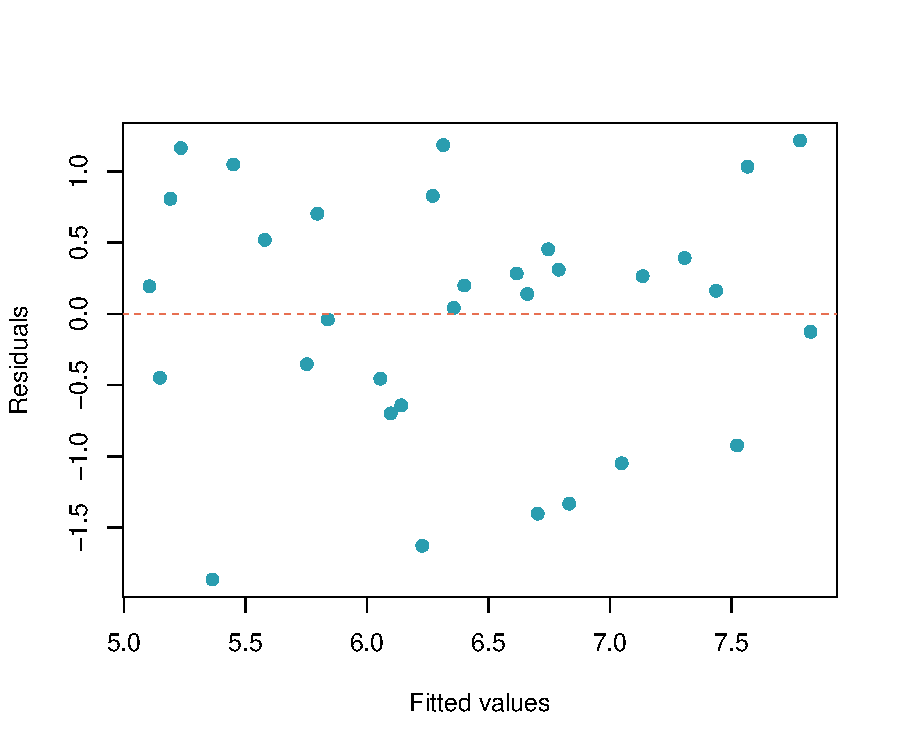
\includegraphics[keepaspectratio]{Homework_quarto_doc_files/figure-pdf/unnamed-chunk-3-2.pdf}}

\subsubsection{2. Running tests}\label{running-tests}

\begin{Shaded}
\begin{Highlighting}[]
\CommentTok{\# Pearson\textquotesingle{}s correlation coefficient test {-}{-}{-}{-}}
\FunctionTok{cor.test}\NormalTok{(kelp}\SpecialCharTok{$}\NormalTok{temp\_c, }
\NormalTok{         kelp}\SpecialCharTok{$}\NormalTok{kelp\_elong, }
         \AttributeTok{method =} \StringTok{"pearson"}\NormalTok{)}
\end{Highlighting}
\end{Shaded}

\begin{verbatim}

    Pearson's product-moment correlation

data:  kelp$temp_c and kelp$kelp_elong
t = -5.189, df = 30, p-value = 1.366e-05
alternative hypothesis: true correlation is not equal to 0
95 percent confidence interval:
 -0.8359665 -0.4460157
sample estimates:
       cor 
-0.6877489 
\end{verbatim}

Linearity was assessed visually using a scatterplot of temperature
vs.~elongation rate with a fitted regression line. Normality of
residuals was checked using a Q-Q plot and homoscedasticity was assessed
using a residuals vs.~fitted values plot. The scatterplot (in part b)
suggests a reasonably linear relationship, the Q-Q plot shows residuals
falling close to the reference line, and the residuals vs.~fitted plot
shows no obvious trend. All assumptions appear reasonably satisfied.

\subsection{d.~Results communication}\label{d.-results-communication}

To evaluate the strength of the relationship between temperature and
giant kelp frond elongation rate I used a Pearson's correlation
coefficient. This tests was an appropriate choice because both variables
are continuous and the scatterplot suggested a linear relationship
between them.

Temperature was a significant negative predictor of giant kelp frond
elongation rate (r = -0.69, p \textless{} 0.001 , R² = 0.473). As
seawater temperature increased, kelp fronds grew more slowly, suggesting
that warmer water conditions are affect Macrocystis pyrifera and inhibit
its growth. This pattern is consistent with what we know about kelp
ecology, giant kelp thrives in cold, nutrient-rich water, and elevated
temperatures likely symbolize conditions such as reduced upwelling that
limit the nutrients available for growth.

\subsection{e. Test implications}\label{e.-test-implications}

Our analysis found a strong negative relationship between seawater
temperature and giant kelp frond elongation rate, meaning kelp grows
significantly slower as water temperatures rise. This is very concerning
given ongoing ocean warming trends. If temperatures continue to
increase, we should expect noticeable declines in kelp growth rates,
which could have cascading effects on the broader kelp forest ecosystem.
I'd recommend to prioritize monitoring sites where temperatures are
already at the higher end of the range we observed, as those are likely
the most at-risk locations for growth suppression.

\subsection{f.~Double check my own
work}\label{f.-double-check-my-own-work}

\begin{Shaded}
\begin{Highlighting}[]
\CommentTok{\# Simple linear regression {-}{-}{-}{-}}
\FunctionTok{summary}\NormalTok{(kelp\_model)}
\end{Highlighting}
\end{Shaded}

\begin{verbatim}

Call:
lm(formula = kelp_elong ~ temp_c, data = kelp)

Residuals:
    Min      1Q  Median      3Q     Max 
-1.8643 -0.5017  0.1790  0.5659  1.2177 

Coefficients:
            Estimate Std. Error t value Pr(>|t|)    
(Intercept) 14.08645    1.49219   9.440 1.72e-10 ***
temp_c      -0.43179    0.08321  -5.189 1.37e-05 ***
---
Signif. codes:  0 '***' 0.001 '**' 0.01 '*' 0.05 '.' 0.1 ' ' 1

Residual standard error: 0.8665 on 30 degrees of freedom
Multiple R-squared:  0.473, Adjusted R-squared:  0.4554 
F-statistic: 26.93 on 1 and 30 DF,  p-value: 1.366e-05
\end{verbatim}

Both Pearson's correlation and simple linear regression led to the same
decision to reject the null hypothesis, confirming that temperature is a
significant predictor of giant kelp frond elongation rate. Pearson's
correlation quantified the strength and direction of the linear
relationship between temperature (°C) and elongation rate (cm/day)
through the r value, while linear regression provided the slope and R²
to describe how much of the variation in elongation rate is explained by
temperature. Both tests agree that as temperature increases, elongation
rate decreases, and together they reinforce the same biological
conclusion --- just from slightly different analytical angles, with
correlation focused on association strength and regression focused on
the nature and predictive power of the relationship.

\section{Problem 2. Personal data}\label{problem-2.-personal-data}

\subsection{a. Updating
visualizations}\label{a.-updating-visualizations}

\begin{Shaded}
\begin{Highlighting}[]
\CommentTok{\# creating new object called my\_data\_clean}
\NormalTok{my\_data\_clean }\OtherTok{\textless{}{-}}\NormalTok{ my\_data }\SpecialCharTok{|\textgreater{}}
\CommentTok{\# cleaning column names so only lowercase and underscores are used}
\FunctionTok{clean\_names}\NormalTok{() }\SpecialCharTok{|\textgreater{}}
  \FunctionTok{mutate}\NormalTok{(}\AttributeTok{duration\_sec =} \FunctionTok{as.numeric}\NormalTok{(}\FunctionTok{ms}\NormalTok{(duration\_mm\_ss)))}
\end{Highlighting}
\end{Shaded}

\begin{Shaded}
\begin{Highlighting}[]
\CommentTok{\# define mm:ss label format}
\NormalTok{mmss\_format }\OtherTok{\textless{}{-}} \ControlFlowTok{function}\NormalTok{(x) }\FunctionTok{sprintf}\NormalTok{(}\StringTok{"\%d:\%02d"}\NormalTok{, x }\SpecialCharTok{\%/\%} \DecValTok{60}\NormalTok{, x }\SpecialCharTok{\%\%} \DecValTok{60}\NormalTok{)}
\CommentTok{\# base layer: gpplot}
\FunctionTok{ggplot}\NormalTok{(}\AttributeTok{data =}\NormalTok{ my\_data\_clean, }
       \CommentTok{\# x{-}axis: trial number}
       \CommentTok{\# y{-}axis: duration}
       \AttributeTok{mapping =} \FunctionTok{aes}\NormalTok{(}\AttributeTok{x =} \FunctionTok{factor}\NormalTok{(trial\_number), }
                     \AttributeTok{y =}\NormalTok{ duration\_sec, }
                     \AttributeTok{color =} \FunctionTok{factor}\NormalTok{(trial\_number))) }\SpecialCharTok{+} 
  \CommentTok{\# first{-}layer: jitter horizontally to organize visualization}
  \FunctionTok{geom\_jitter}\NormalTok{(}\AttributeTok{width =} \FloatTok{0.13}\NormalTok{,}
              \AttributeTok{height =} \DecValTok{0}\NormalTok{,}
              \AttributeTok{size =} \FloatTok{2.5}\NormalTok{) }\SpecialCharTok{+}
  \CommentTok{\# mean points on graph}
  \FunctionTok{stat\_summary}\NormalTok{(}\AttributeTok{fun =}\NormalTok{ mean, }\CommentTok{\# calculate average}
               \AttributeTok{geom =} \StringTok{"point"}\NormalTok{,  }\CommentTok{\# display as point}
               \AttributeTok{color =} \StringTok{"\#f2f533"}\NormalTok{, }\CommentTok{\# change color of point}
               \AttributeTok{shape =} \DecValTok{13}\NormalTok{, }\CommentTok{\# change shape of point}
               \AttributeTok{size =} \DecValTok{10}\NormalTok{) }\SpecialCharTok{+}
  \CommentTok{\# standard deviation error bars}
  \FunctionTok{stat\_summary}\NormalTok{(}\AttributeTok{fun.data =}\NormalTok{ mean\_sdl, , }\CommentTok{\# calculate standard deviation}
               \AttributeTok{fun.args =} \FunctionTok{list}\NormalTok{(}\AttributeTok{mult =} \FloatTok{0.5}\NormalTok{), }\CommentTok{\# tighter view of variability}
               \AttributeTok{geom =} \StringTok{"errorbar"}\NormalTok{, }\CommentTok{\# adding error{-}bar}
               \AttributeTok{width =} \FloatTok{0.4}\NormalTok{, }\CommentTok{\# changing width}
               \AttributeTok{color =} \StringTok{"\#2b2b2b"}\NormalTok{) }\SpecialCharTok{+} \CommentTok{\# changing color}
  \CommentTok{\# assigning colors to trial 1 and trial 2 }
  \FunctionTok{scale\_color\_manual}\NormalTok{(}\AttributeTok{values =} \FunctionTok{c}\NormalTok{(}\StringTok{"1"} \OtherTok{=} \StringTok{"\#19e36a"}\NormalTok{,}
                                \StringTok{"2"} \OtherTok{=} \StringTok{"\#7836b5"}\NormalTok{)) }\SpecialCharTok{+}
  \CommentTok{\# assigning a new and organized scale for y{-}axis }
  \FunctionTok{scale\_y\_continuous}\NormalTok{(}
    \AttributeTok{breaks =} \FunctionTok{seq}\NormalTok{(}\DecValTok{600}\NormalTok{, }\FunctionTok{max}\NormalTok{(my\_data\_clean}\SpecialCharTok{$}\NormalTok{duration\_sec, }\AttributeTok{na.rm =} \ConstantTok{TRUE}\NormalTok{), }\AttributeTok{by =} \DecValTok{60}\NormalTok{),}
    \AttributeTok{minor\_breaks =} \FunctionTok{seq}\NormalTok{(}\DecValTok{600}\NormalTok{, }\FunctionTok{max}\NormalTok{(my\_data\_clean}\SpecialCharTok{$}\NormalTok{duration\_sec, }\AttributeTok{na.rm =} \ConstantTok{TRUE}\NormalTok{), }\AttributeTok{by =} \DecValTok{30}\NormalTok{),}
    \AttributeTok{labels =}\NormalTok{ mmss\_format}
\NormalTok{  ) }\SpecialCharTok{+}
  \CommentTok{\# adjusting plot (decreasing space in between categories and plot borders)}
  \FunctionTok{scale\_x\_discrete}\NormalTok{(}\AttributeTok{expand =} \FunctionTok{expansion}\NormalTok{(}\AttributeTok{add =} \FloatTok{0.7}\NormalTok{, }\AttributeTok{mult =} \FloatTok{0.05}\NormalTok{)) }\SpecialCharTok{+}
  \CommentTok{\# changing theme from default}
  \FunctionTok{theme\_bw}\NormalTok{(}\AttributeTok{base\_family =} \StringTok{"serif"}\NormalTok{) }\SpecialCharTok{+}
   \CommentTok{\# changing panel and plot background}
  \FunctionTok{theme}\NormalTok{(}
    \AttributeTok{panel.background =} \FunctionTok{element\_rect}\NormalTok{(}\AttributeTok{fill =} \StringTok{"lightblue"}\NormalTok{),}
    \AttributeTok{plot.background =} \FunctionTok{element\_rect}\NormalTok{(}\AttributeTok{fill =} \StringTok{"transparent"}\NormalTok{, }\AttributeTok{color =} \ConstantTok{NA}\NormalTok{)}
\NormalTok{  ) }\SpecialCharTok{+}
  \CommentTok{\# taking out the minor grid}
  \FunctionTok{theme}\NormalTok{(}\AttributeTok{panel.grid.minor =} \FunctionTok{element\_blank}\NormalTok{()) }\SpecialCharTok{+}
  \CommentTok{\# taking out major grid }
  \FunctionTok{theme}\NormalTok{(}\AttributeTok{panel.grid.major =} \FunctionTok{element\_blank}\NormalTok{()) }\SpecialCharTok{+}
  \CommentTok{\# taking out legend }
  \FunctionTok{theme}\NormalTok{(}\AttributeTok{legend.position =} \StringTok{"none"}\NormalTok{) }\SpecialCharTok{+}
  \CommentTok{\# adjusting title position}
  \FunctionTok{theme}\NormalTok{(}\AttributeTok{plot.title =} \FunctionTok{element\_text}\NormalTok{(}\AttributeTok{hjust =} \FloatTok{0.5}\NormalTok{)) }\SpecialCharTok{+}
  \CommentTok{\# adjusting subtitle position}
  \FunctionTok{theme}\NormalTok{(}\AttributeTok{plot.subtitle =} \FunctionTok{element\_text}\NormalTok{(}\AttributeTok{hjust =} \FloatTok{0.5}\NormalTok{)) }\SpecialCharTok{+}
  \CommentTok{\# adding title and labeling to x{-} and y{-}axis}
  \FunctionTok{labs}\NormalTok{(}\AttributeTok{x =} \StringTok{"Trial Number"}\NormalTok{,}
       \AttributeTok{y =} \StringTok{"Duration (mm:ss)"}\NormalTok{,}
       \AttributeTok{title =} \StringTok{"Travel Time Analysis: Trial \# and Duration"}\NormalTok{, }
       \AttributeTok{subtitle =} \StringTok{"Latest observation; 5/26/2026"}\NormalTok{)}
\end{Highlighting}
\end{Shaded}

\pandocbounded{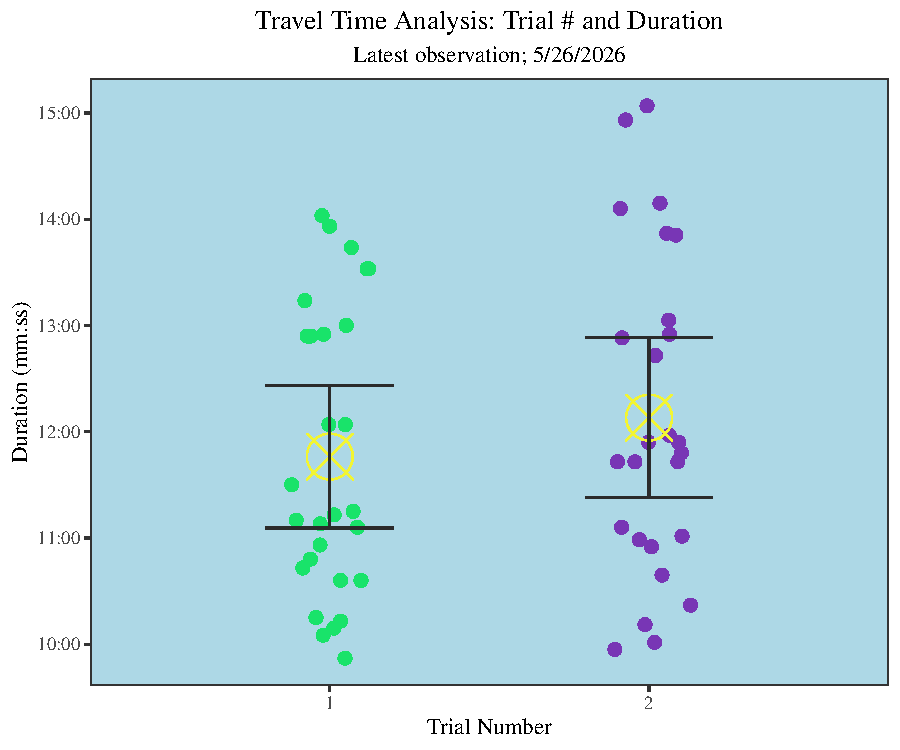
\includegraphics[keepaspectratio]{Homework_quarto_doc_files/figure-pdf/unnamed-chunk-7-1.pdf}}

\begin{Shaded}
\begin{Highlighting}[]
\CommentTok{\# base layer ggplot}
\FunctionTok{ggplot}\NormalTok{(}\AttributeTok{data =}\NormalTok{ my\_data\_clean,}
       \CommentTok{\# x{-}axis = wind speed}
       \CommentTok{\# \# y{-}axis = direction of trip}
       \CommentTok{\# \# color varies by direction of trip}
      \FunctionTok{aes}\NormalTok{(}\AttributeTok{x =}\NormalTok{ wind\_speed\_mph,}
                     \AttributeTok{y =}\NormalTok{ duration\_sec,}
                     \AttributeTok{color =}\NormalTok{ direction\_of\_trip)) }\SpecialCharTok{+}
  \CommentTok{\# adding points}
  \FunctionTok{geom\_point}\NormalTok{(}\AttributeTok{size =} \DecValTok{4}\NormalTok{, }\AttributeTok{alpha =} \FloatTok{0.8}\NormalTok{) }\SpecialCharTok{+}
  \CommentTok{\# adding a regression line for both plots}
  \FunctionTok{geom\_smooth}\NormalTok{(}\AttributeTok{method =} \StringTok{"lm"}\NormalTok{, }\AttributeTok{se =} \ConstantTok{FALSE}\NormalTok{) }\SpecialCharTok{+}
  \CommentTok{\# splitting into two graphs (one per category)}
  \FunctionTok{facet\_wrap}\NormalTok{(}\SpecialCharTok{\textasciitilde{}}\NormalTok{ direction\_of\_trip) }\SpecialCharTok{+}
  \CommentTok{\# assigning a new and organized scale for the y{-}axis }
  \FunctionTok{scale\_y\_continuous}\NormalTok{(}
    \AttributeTok{breaks =} \FunctionTok{seq}\NormalTok{(}\DecValTok{600}\NormalTok{, }\FunctionTok{max}\NormalTok{(my\_data\_clean}\SpecialCharTok{$}\NormalTok{duration\_sec, }\AttributeTok{na.rm =} \ConstantTok{TRUE}\NormalTok{), }\AttributeTok{by =} \DecValTok{60}\NormalTok{),}
    \AttributeTok{minor\_breaks =} \FunctionTok{seq}\NormalTok{(}\DecValTok{600}\NormalTok{, }\FunctionTok{max}\NormalTok{(my\_data\_clean}\SpecialCharTok{$}\NormalTok{duration\_sec, }
                                \AttributeTok{na.rm =} \ConstantTok{TRUE}\NormalTok{), }\AttributeTok{by =} \DecValTok{30}\NormalTok{),}
    \AttributeTok{labels =}\NormalTok{ mmss\_format}
\NormalTok{  ) }\SpecialCharTok{+}
   \CommentTok{\# assigning colors for each categories}
  \FunctionTok{scale\_color\_manual}\NormalTok{(}\AttributeTok{values =} \FunctionTok{c}\NormalTok{(}\StringTok{"home to UCSB"} \OtherTok{=} \StringTok{"\#fc5538"}\NormalTok{,}
                                \StringTok{"UCSB to home"} \OtherTok{=} \StringTok{"\#7836b5"}\NormalTok{)) }\SpecialCharTok{+}
   \CommentTok{\# changing theme from default}
  \FunctionTok{theme\_light}\NormalTok{(}\AttributeTok{base\_family =} \StringTok{"serif"}\NormalTok{) }\SpecialCharTok{+}
  \CommentTok{\# changing panel and plot background}
  \FunctionTok{theme}\NormalTok{(}
    \AttributeTok{panel.background =} \FunctionTok{element\_rect}\NormalTok{(}\AttributeTok{fill =} \StringTok{"\#bdffd7"}\NormalTok{),}
    \AttributeTok{plot.background =} \FunctionTok{element\_rect}\NormalTok{(}\AttributeTok{fill =} \StringTok{"transparent"}\NormalTok{, }\AttributeTok{color =} \ConstantTok{NA}\NormalTok{)}
\NormalTok{  ) }\SpecialCharTok{+}
  \CommentTok{\# labeling x{-} and y{-}axis and adding title}
  \FunctionTok{labs}\NormalTok{(}\AttributeTok{title =} \StringTok{"Travel Time Analysis: Wind \& Duration"}\NormalTok{,}
       \AttributeTok{subtitle =} \StringTok{"Latest observation; 5/26/2026"}\NormalTok{,}
       \AttributeTok{x =} \StringTok{"Wind Speed (mph)"}\NormalTok{,}
       \AttributeTok{y =} \StringTok{"Duration (mm:ss)"}\NormalTok{) }\SpecialCharTok{+}
  \CommentTok{\# taking out the minor grid}
  \FunctionTok{theme}\NormalTok{(}\AttributeTok{panel.grid.minor =} \FunctionTok{element\_blank}\NormalTok{()) }\SpecialCharTok{+}
  \CommentTok{\# taking out major grid }
  \FunctionTok{theme}\NormalTok{(}\AttributeTok{panel.grid.major =} \FunctionTok{element\_blank}\NormalTok{()) }\SpecialCharTok{+}
  \CommentTok{\# taking out legend }
  \FunctionTok{theme}\NormalTok{(}\AttributeTok{legend.position =} \StringTok{"none"}\NormalTok{) }\SpecialCharTok{+}
  \CommentTok{\# adjusting title position}
  \FunctionTok{theme}\NormalTok{(}\AttributeTok{plot.title =} \FunctionTok{element\_text}\NormalTok{(}\AttributeTok{hjust =} \FloatTok{0.5}\NormalTok{)) }\SpecialCharTok{+}
  \CommentTok{\# adjusting subtitle position}
  \FunctionTok{theme}\NormalTok{(}\AttributeTok{plot.subtitle =} \FunctionTok{element\_text}\NormalTok{(}\AttributeTok{hjust =} \FloatTok{0.5}\NormalTok{)) }\SpecialCharTok{+}
  \CommentTok{\# adjusting facet\_wrap text and color}
  \FunctionTok{theme}\NormalTok{(}
  \AttributeTok{strip.text =} \FunctionTok{element\_text}\NormalTok{(}\AttributeTok{size =} \DecValTok{12}\NormalTok{, }\AttributeTok{color =} \StringTok{"white"}\NormalTok{),}
  \AttributeTok{strip.background =} \FunctionTok{element\_rect}\NormalTok{(}\AttributeTok{fill =} \StringTok{"\#8e9e95"}\NormalTok{)) }\SpecialCharTok{+}
  \CommentTok{\# adjusting x{-} and y{-}axis text}
  \FunctionTok{theme}\NormalTok{(}\AttributeTok{axis.title =} \FunctionTok{element\_text}\NormalTok{(}\AttributeTok{size =} \DecValTok{12}\NormalTok{))}
\end{Highlighting}
\end{Shaded}

\pandocbounded{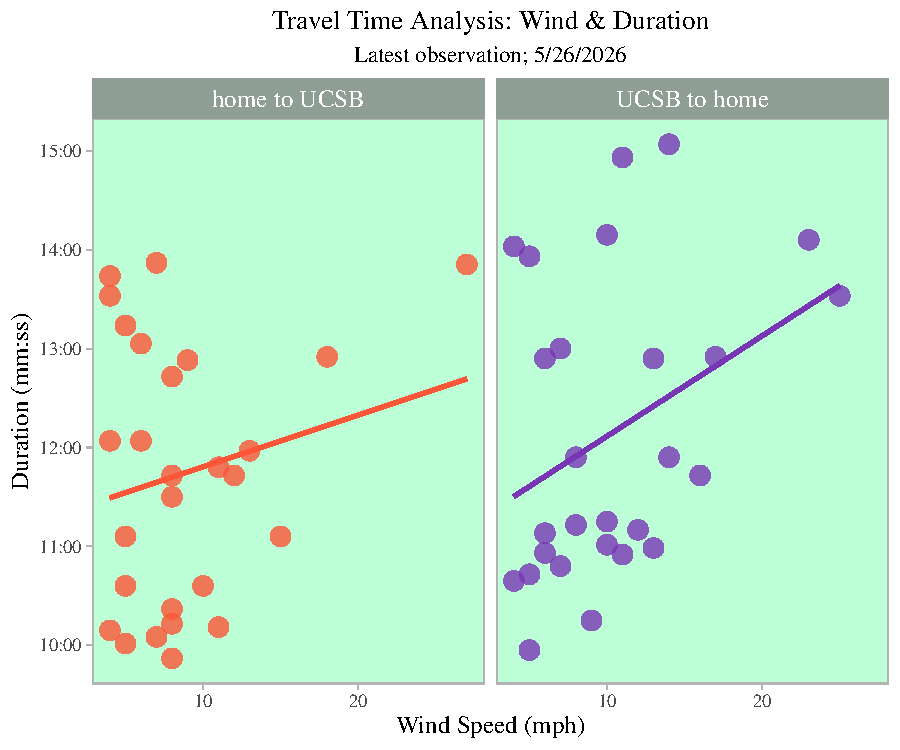
\includegraphics[keepaspectratio]{Homework_quarto_doc_files/figure-pdf/unnamed-chunk-8-1.pdf}}

\subsection{b. Captions}\label{b.-captions}

Figure 1. Scatter plot with mean travel duration for trial number 1 and
2 and error bars displaying \(\pm\) 0.5 standard deviations around the
mean. Individual observation points in each trial are denoted by x-axis
(1,2) as well as colors (trial 1: green, trial 2: purple). Trial number
averages are denoted by the yellow circles with X's going through. Error
bars display the 95\% confidence interval around each regional mean.
Data source: Michael Torbensen. 2026. Average bike duration spreadsheet.

Figure 2. Two separate panels for travel direction show scatter plots
with a regression line modeling the average relationship between
duration (y-axis) and wind speed (x-axis). The first panel (home to
UCSB) features red points indicating individual observations as well as
a red regression line. The second panel (UCSB to home) features purple
points indicating observations as well as a purple regression line. Data
source: Michael Torbensen. 2026. Average bike duration spreadsheet.

\section{Problem 3. Affective
visualization}\label{problem-3.-affective-visualization}

\subsection{a. Idea for affective
visualization}\label{a.-idea-for-affective-visualization}

For my affective visualization, I was thinking of representing mostly
all of my data with two bikes using the wheels as a place to represent
my individual observations. The separate bikes will represent all data
points that fall on either trial number one or two (categorical data).
The rear wheel will represent home to UCSB data observations and the
front wheel will represent UCSB to home observations (categorical data).
Within the tires, each spoke will represent wind speed (width of spoke),
travel duration (length of spoke), and number of stop lights (color of
spoke). Also, I'm thinking of adding a sheen/gloss to the spoke with the
quickest trip and the slowest trip will be a little transparent.

\subsection{b. Sketch for
visualization}\label{b.-sketch-for-visualization}

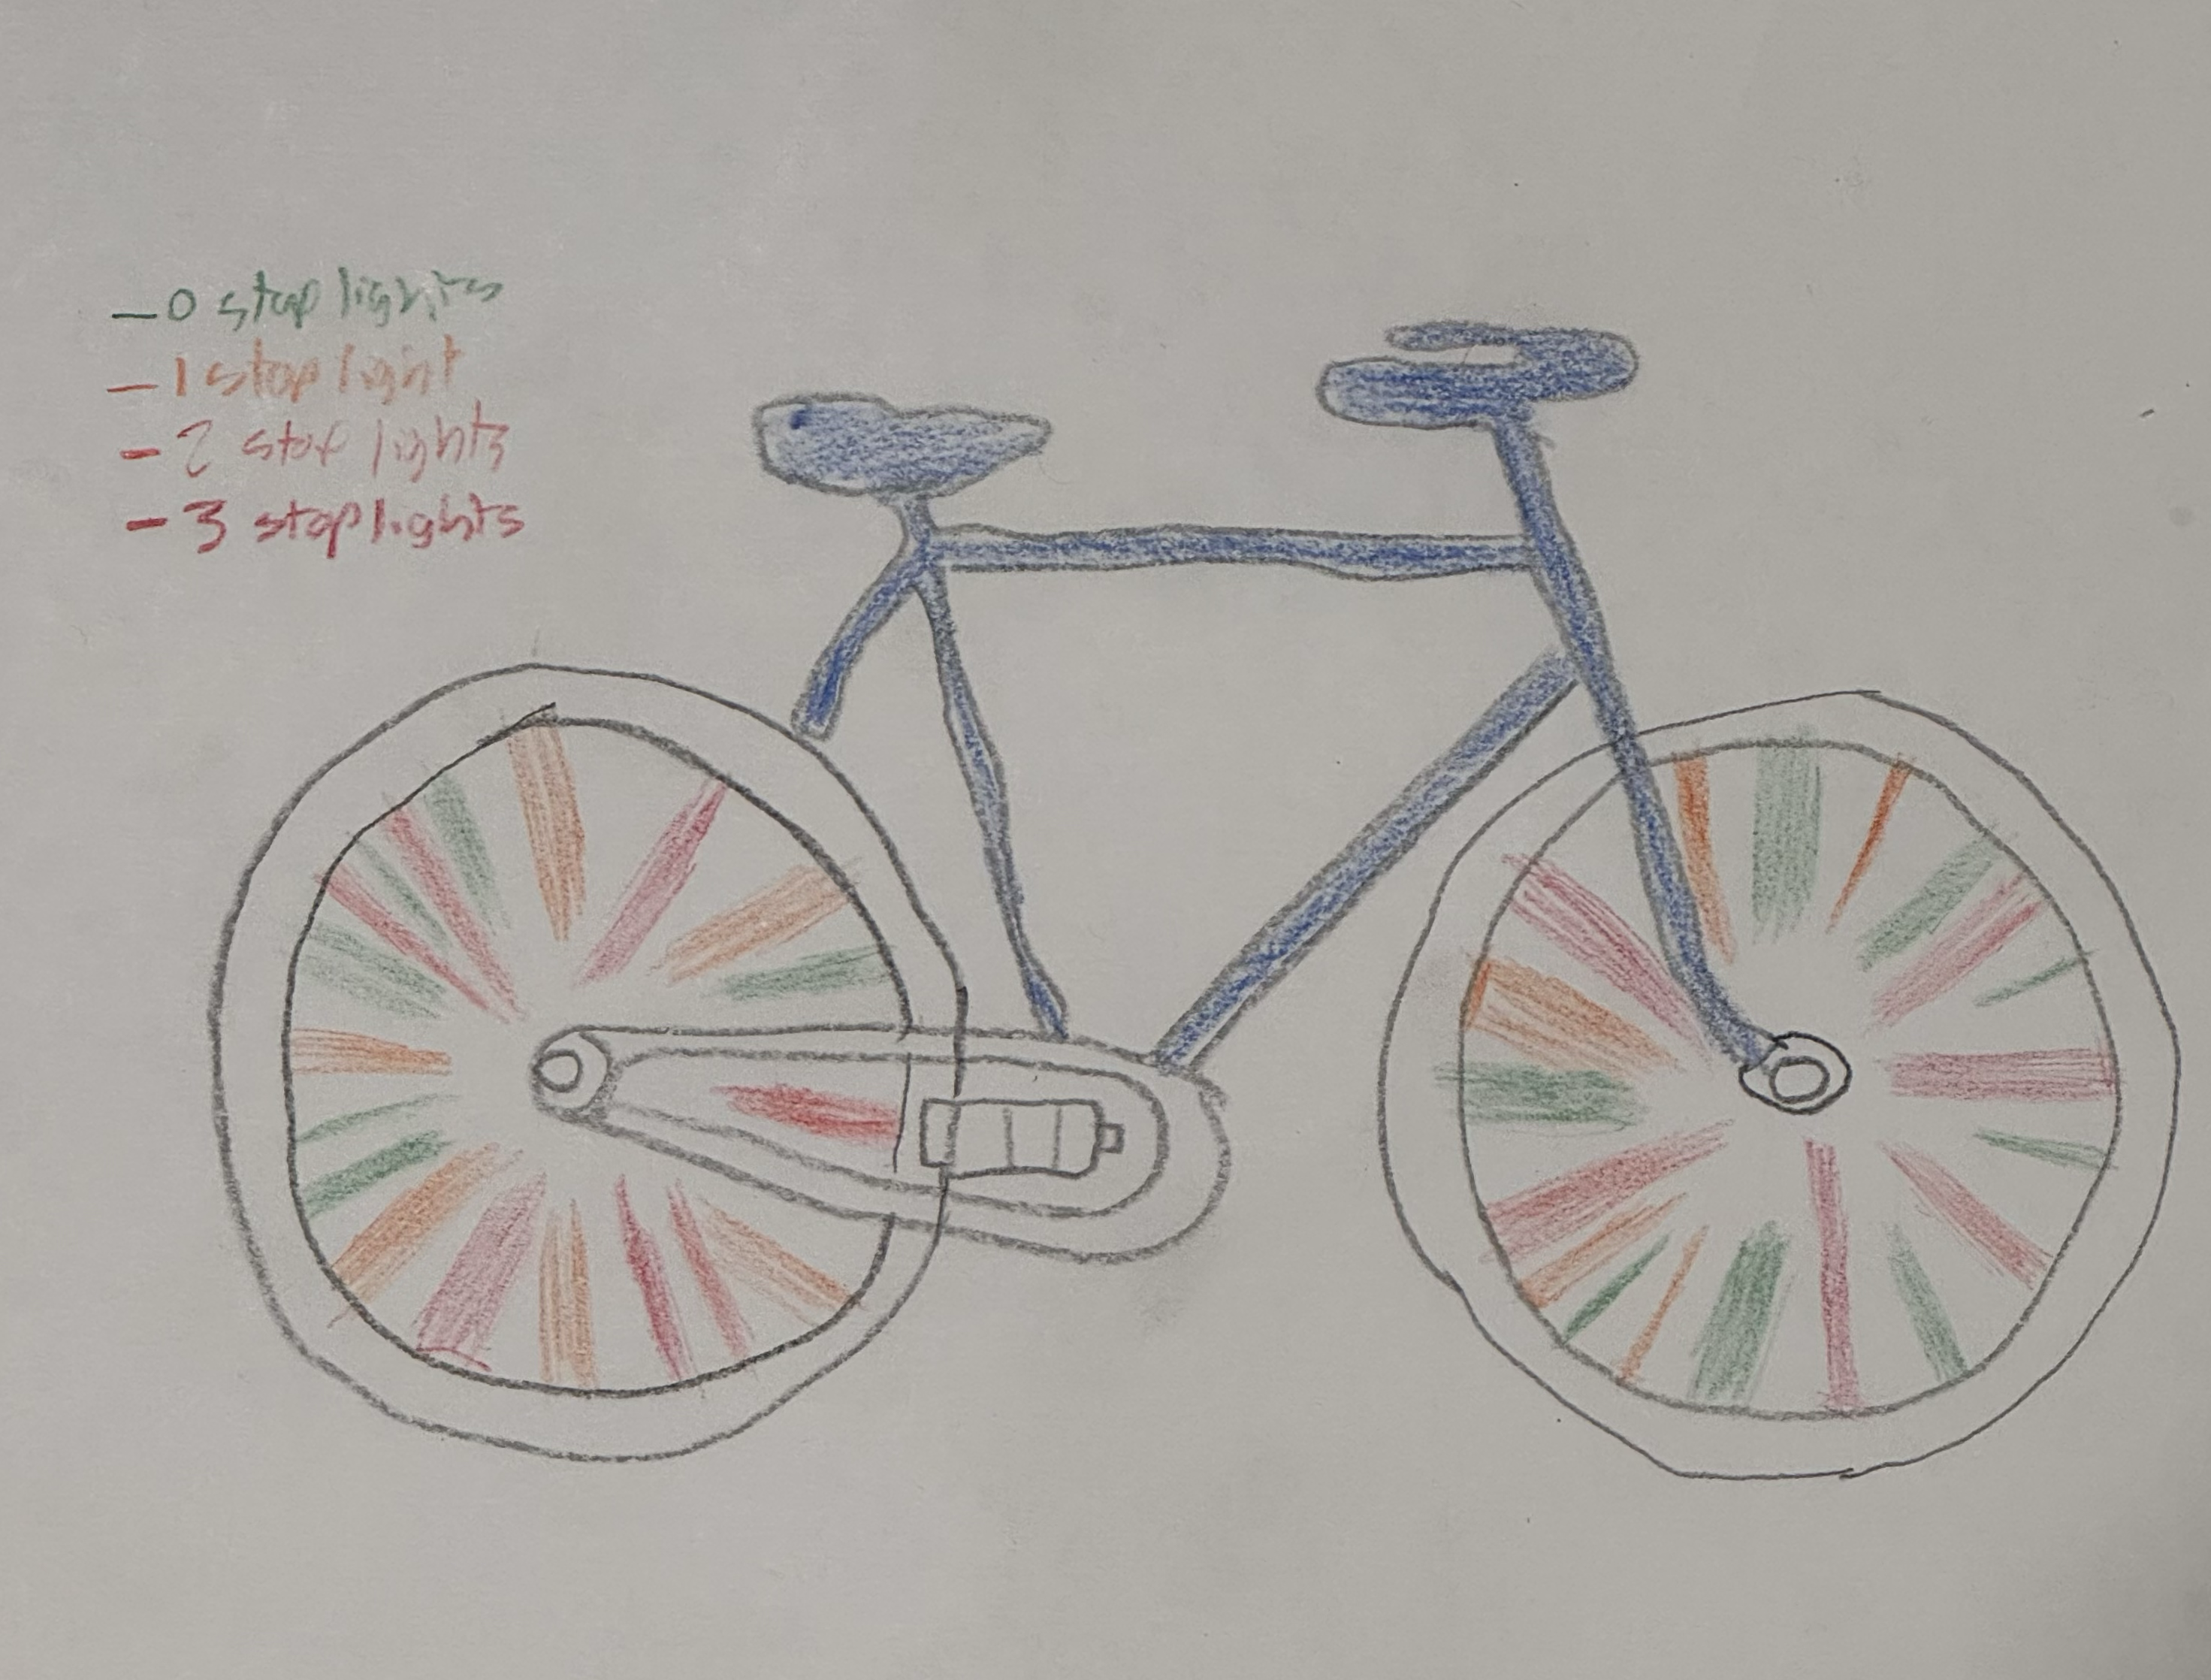
\includegraphics[width=9.81in,height=\textheight,keepaspectratio]{images/sketch.png}

\subsection{c.~Draft of visualization}\label{c.-draft-of-visualization}

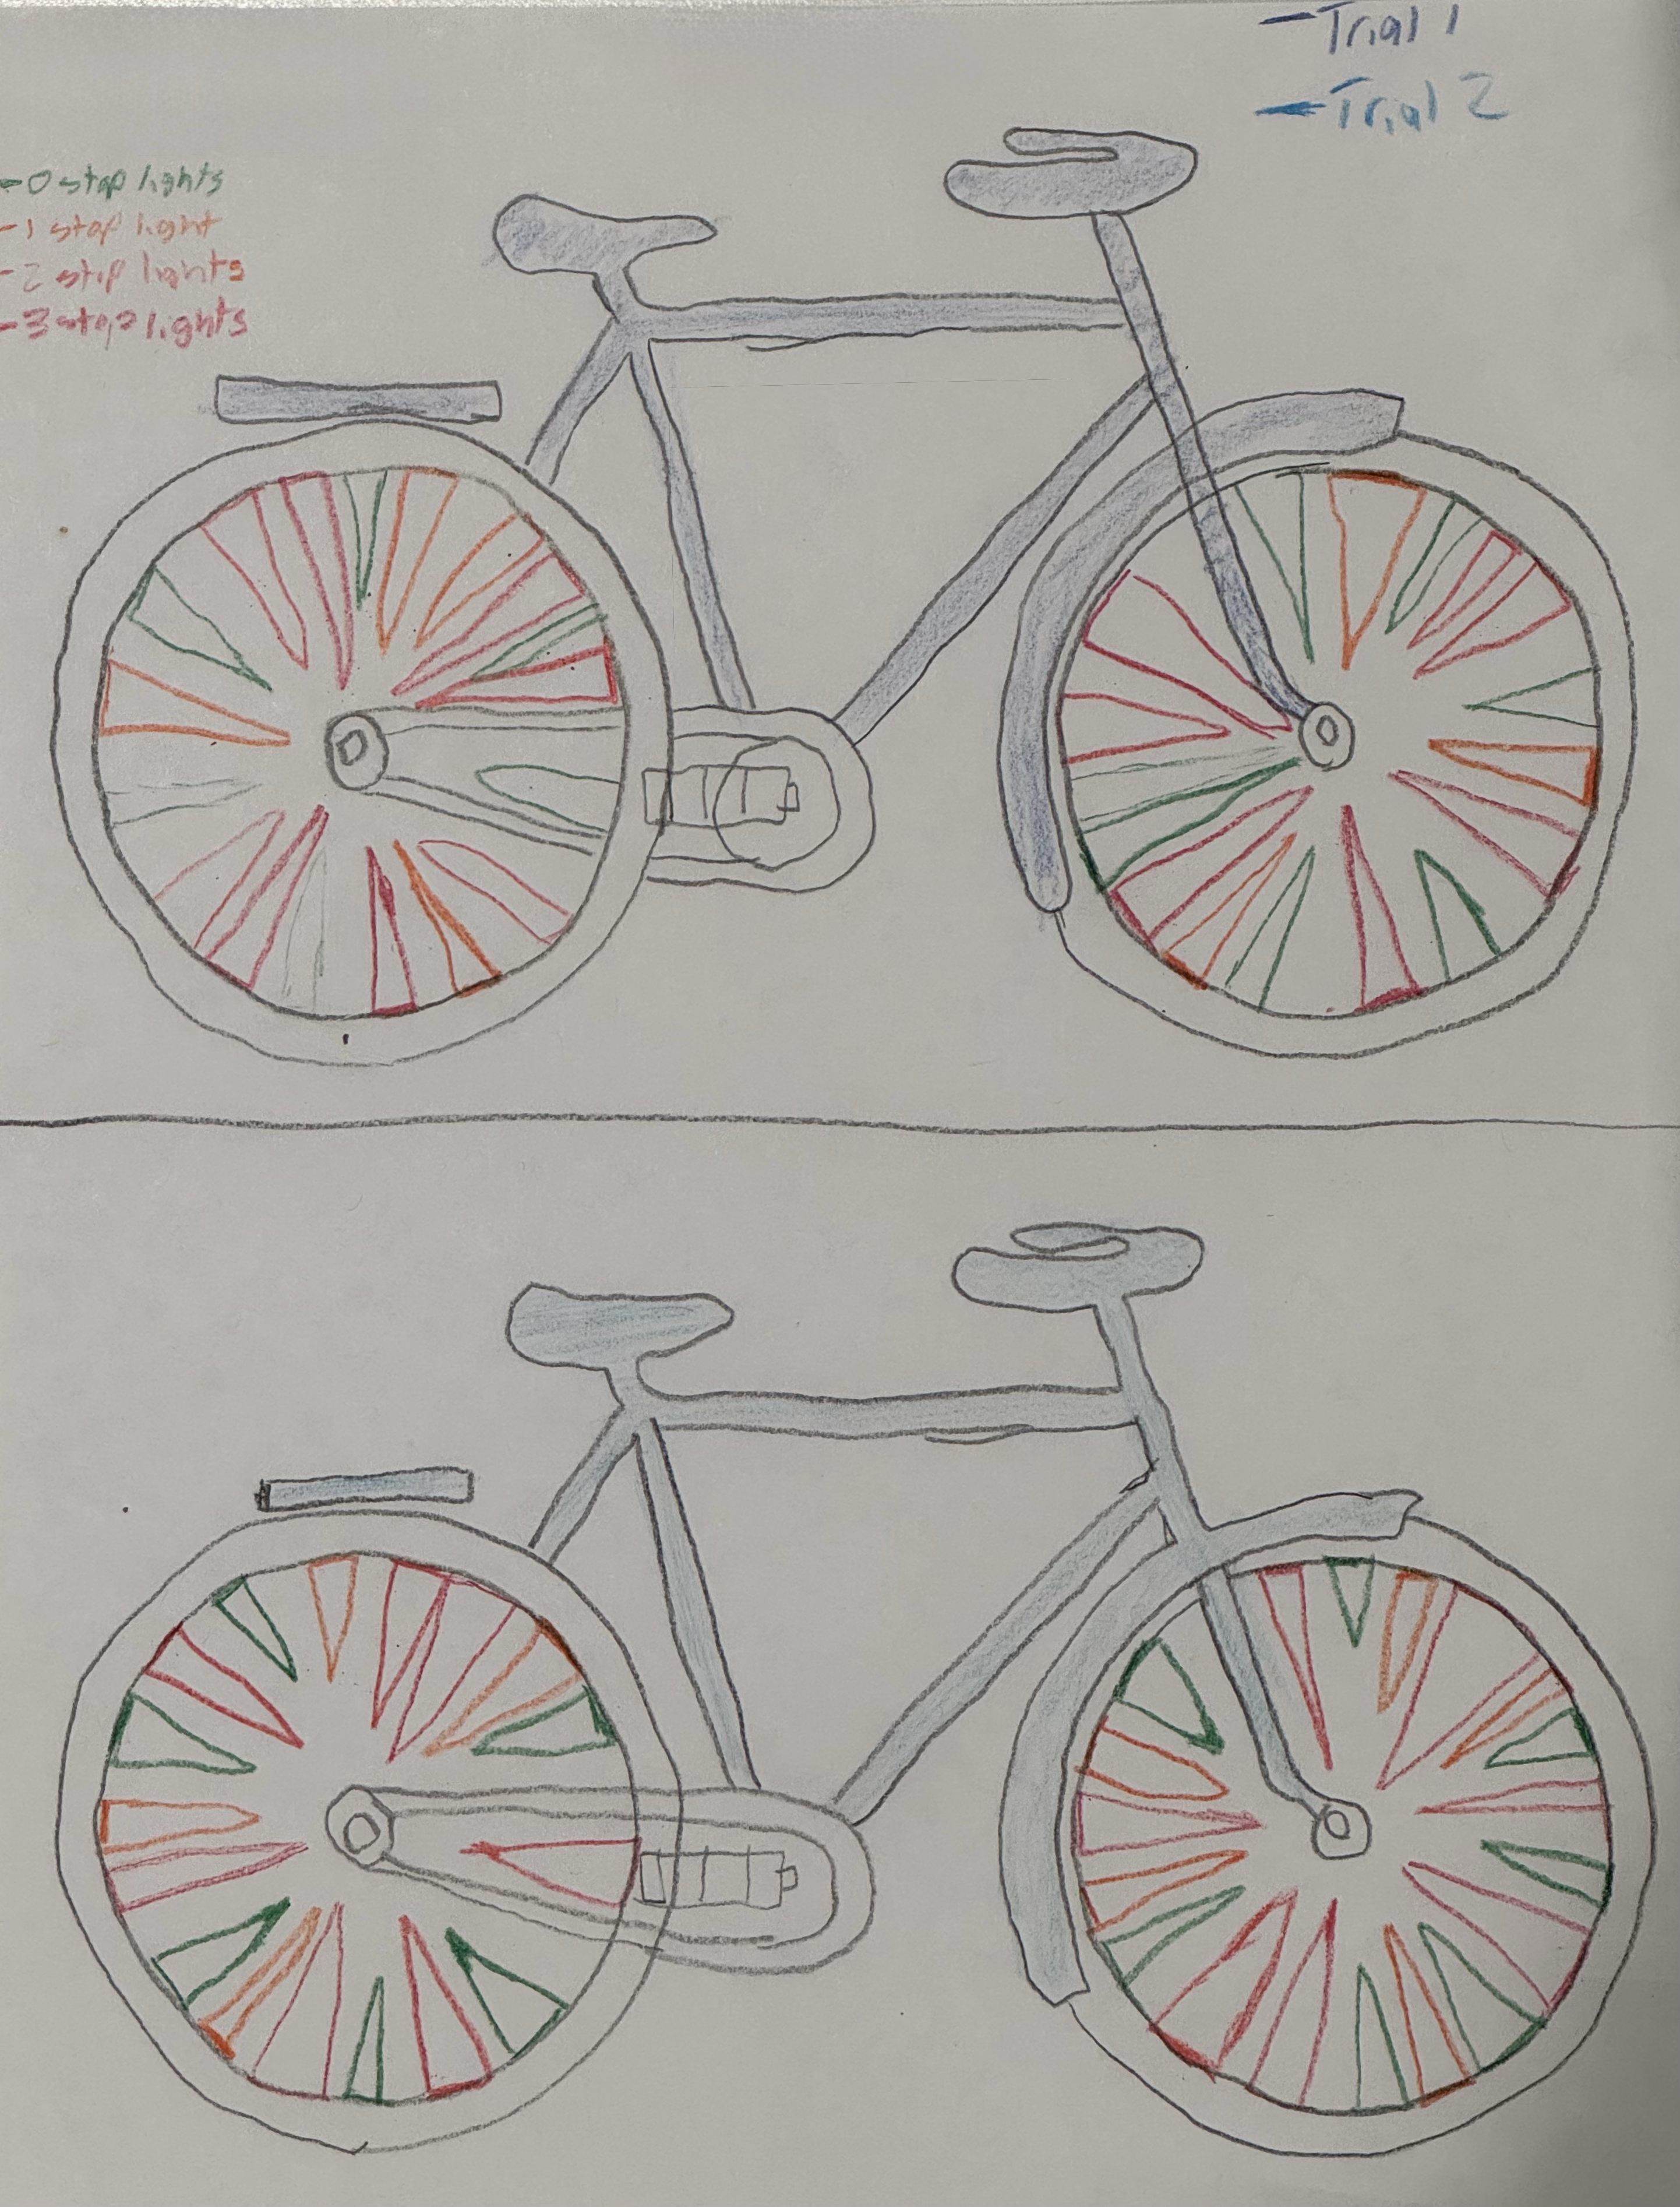
\includegraphics[width=0.75\linewidth,height=\textheight,keepaspectratio]{images/bike_visual.png}

\subsection{d.~Artist statement}\label{d.-artist-statement}

I enjoy getting to my destinations as fast as possible and learning what
variables makes me slower and what variables makes me faster. So, I have
created a two panel plot that expresses two different categorical
variables and 3 different continuous variables. I will be using colored
pencils on a blank sheet of white paper to create my final drafted
drawing.

\subsection{e. Presentation}\label{e.-presentation}

\href{https://docs.google.com/presentation/d/1Pwn96klhM3I_SVNqkeeJASpArRlIhMYD2BLW1zIHzIE/present}{View
Presentation}

\section{Problem 4. Statistical
critique}\label{problem-4.-statistical-critique}

\subsection{a. Revisit and summarize}\label{a.-revisit-and-summarize}

In this paper, the author is wondering how effective re-connected
floodplains are at de-nitrifying bodies of water that are useful to
humans and other biological communities. Out of the tests conducted,
analysis of variance (ANOVA) is the main test that the author used.

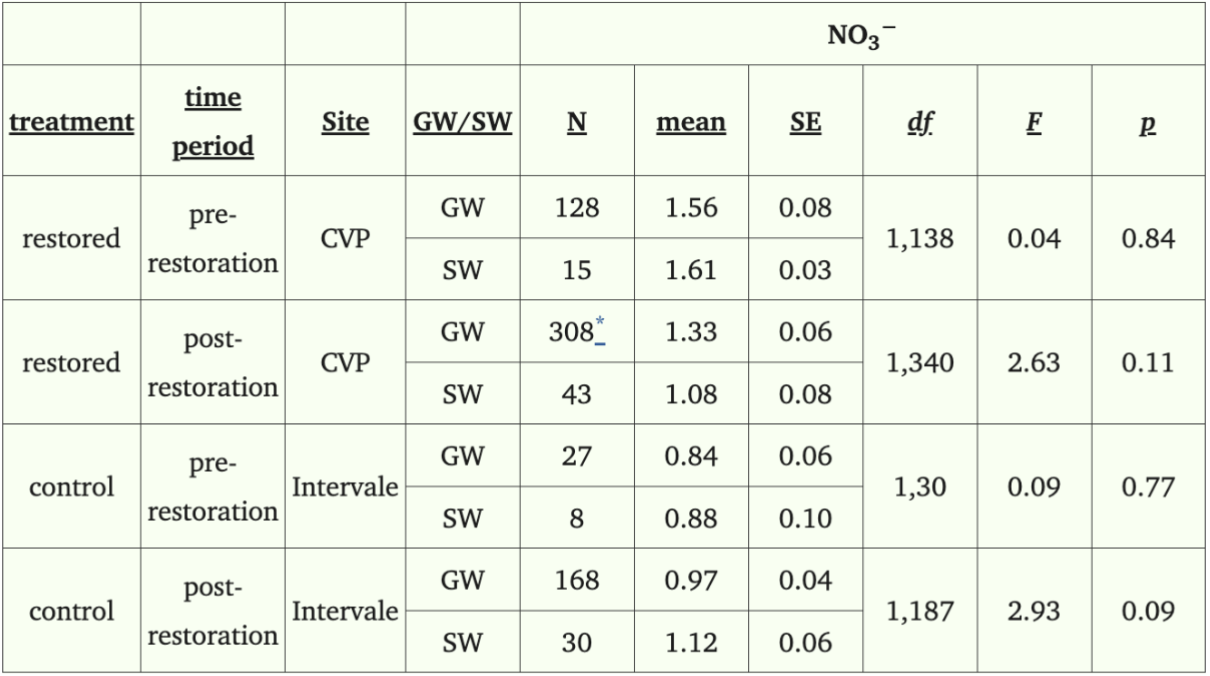
\includegraphics[width=4.03in,height=\textheight,keepaspectratio]{images/ANOVA.png}

\subsection{b. Visual Clarity}\label{b.-visual-clarity}

The table clearly shows the results of the ANOVA tests by including the
key statistical components needed for interpretation: degrees of
freedom, F-statistic, and p-value. The inclusion of N (sample size),
mean, and SE (standard error) alongside the test statistics is also
useful because it gives the reader context for the raw data underlying
each comparison, rather than just isolating the test results.

\subsection{c.~Aesthetic clarity}\label{c.-aesthetic-clarity}

The authors handled visual clutter in a way that made the graph legible
but not with outstanding quality. The categories listed in the table are
bold so that each separate category cannot be confused with the other.
Although, all data have the same font style, size, and type. So, if
there is any data that is particularly useful for the validity of the
test results, it cannot be deduced by looking at the graph. That being
said, the organization by treatment, time period, and site makes it easy
to compare across all four ANOVAs.

\subsection{d.~Recommendations}\label{d.-recommendations}

Typically, for an ANOVA test, it's common to mention the sum of squares
(SS) and mean squares (MS) to measure the among-group variation and
within-group variation as this is where the F-statistic and effect size
come from. This would give more information to the reader and increase
clarity and comprehension of the data. Also, since the group sizes are
so large, the SE numbers are very small. If the SE column was replaced
with SD, the spread of the nitrate measurements in each group would be
much more visible and one can judge whether differences between group
means are biologically significant.




\end{document}
